\documentclass[sr]{./../../common/SurferDesc}%%%%%%%%%%%%%%%%%%%%%%%%%%%%%%%%%%%%%%%%%%%%%%%%%%%%%%%%%%%%%%%%%%%%%%%
%
% The document starts here:
%
\begin{document}
\footnotesize
% WeltrekordflŠchen

%%% 1.Tafel

%%%%%%%%%%%%%%%%%%%%%%%%%%%%%

\begin{surferPage}
  \begin{surferTitle}Бартова површ шестог степена са 30 шиљака\end{surferTitle}  

    Након што је Волф Барт конструисао површ шестог степена са максималним бројем 
	сингуларитета, $65$, а два његова докторанта рекордерске површи за веће степене, 
    Барт је почео да се бави питањем највећег броја шиљака на површи одређеног степена.

   Бартова конструкција површи шестог степена са $65$ сингуларитета типа 
    $A_1^{+-}$ (двострука купа) се може прерадити у шиљке, што доводи до њих  $30$: 
    \[P_6 - \alpha \cdot K^3=0,\]
  где су  $P_6$ исте равни симтерија за икосаедар
    као и код других Бартових површи, а $K$ је
    поново једначина јединичне сфере:
    \vspace*{-0.4em}
    \begin{center}
      \begin{tabular}{c@{\ }c@{\ }c@{\ }c}
        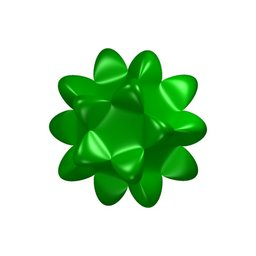
\includegraphics[height=1.2cm]{./../../common/images/barthsextic_30A2}
        &
        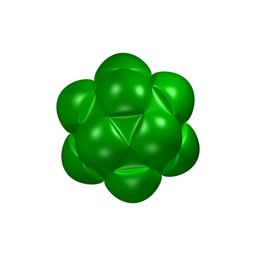
\includegraphics[height=1.2cm]{./../../common/images/barthsextic_30A2_3}
        &
        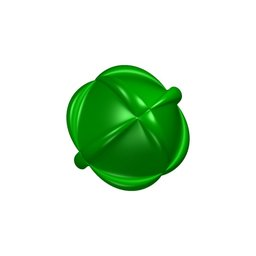
\includegraphics[height=1.2cm]{./../../common/images/barthsextic_30A2_5}
        &
        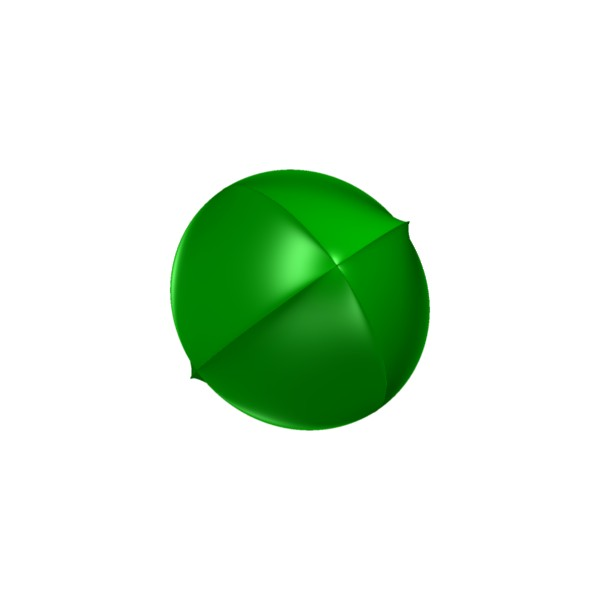
\includegraphics[height=1.2cm]{./../../common/images/barthsextic_30A2_6}
      \end{tabular}
    \end{center}    
    \vspace*{-0.3em}
     Ово представља тренутни светски рекорд за максималан број реалних шиљака за површи шестог степена;
	 максималан број комплексних шиљака је  $36$. 



  \begin{surferText}
     \end{surferText}
\end{surferPage}
%%%%%%%%%%%%%%%%%%%%%%%%%%%%%


\end{document}
%
% end of the document.
%
%%%%%%%%%%%%%%%%%%%%%%%%%%%%%%%%%%%%%%%%%%%%%%%%%%%%%%%%%%%%%%%%%%%%%%%
